\subsection{Kolonnefamiliedatabase}
Cassandra er verktøyet vi skulle bruke for å opprette Kolonnefamiliedatabaser. Fra tidligere hadde vi allerede designet aggregeringene og laget de via spark-shell i Scala, så prossessen var heldigvis rett fram. For alle aggregeringene, inkluderende rådataen, måtte man opprette en ny table/kolonnefamilie i Cassandra med samsvarende kolonnenavn og datatype.

\subsubsection{Opprette keyspace}
Det første må gjøre er å opprette et "keyspace" i Cassandra. Dette tilsvarer en database i MySQL. Her opprettes keyspacet "university" hvor alle kommende tables havner i. Det er viktig å merke seg \lstinline{WITH replication}, siden den bestemmer hvordan datakopier spres utover en klynge. For denne løsning brukes \textit{SimpleStrategy} med \textit{replication factor} av 1. 

\txt{code/milepael6/createNamespace.txt}

Replikasjonsstrategien bestemmer hvordan datakopiene distribueres rundt om i \textit{Cassandra ringen}, der en ring representerer en klynge av noder, også kalt et datasenter. Som en tommelfingelregel brukes SimpleStrategy når man bare har et datasenter, ellers brukes \textit{NetworkTopologyStrategy}. Begge strategiene populerer datasettene node for node med klokken, forskjellen er at SimpleStrategy kun populerer et datasett, mens NetworkTopologyStrategy populererer flere.

\begin{figure}[H]
  \centering
  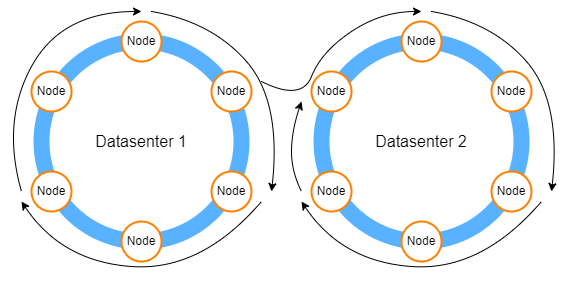
\includegraphics[scale=0.5]{images/milepael6/replicationstrategy.drawio.png}
  \caption{Figuren viser hvordan de to replikasjonsstrategiene distribuerer datakopier utover klyngene. SimpleStrategy vil kun distribuere til datasenter 1, mens NetworkTopologyStrategy vil starte i datasenter 1 og jobbe seg utover datasenter 2.}
\end{figure}

Videre bestemmer replikasjonsfaktoren hvor mange datakopier som skal spres utover klyngen, for eksempel i en klynge med seks noder og replikasjonsfaktor på tre, vil halvparten av nodene være tilgitt en datakopi. På denne måten forsørger man at data er utilgjengelig dersom en node skulle feile. Legg merke til at det ikke er lov til å ha en replikasjonsfaktor større enn antall noder i en klynge. 

I Cassandra tar man også hensyn til noe kalt for \textit{Cassandra consistensy level}, som er minimum antall noder som må annerkjenne lese- og skrive-spørringer før det kan kalles en gyldig operasjon. Dette er en verdi som kan settes selv. Som regel brukes Cassandra verdien \textit{Local Quorum}, som defineres slik: \lstinline{LOCAL_QUORUM = (replication_factor/2) + 1}, denne rundes ned til nærmeste heltall.

\subsubsection{Opprette kolonnefamilier i Cassandra}
Det neste er å opprette selve tabellene i Cassandra via \lstinline{CREATE TABLE} setningen. Her er det viktig å passe på at både kolonnenavn og datatyper stemmer med datasettet, ellers kan man ikke sende dataen videre til Cassandra. I tillegg krever Cassandra minst én \textit{primærnøkkel}, noe som var problamtisk da det opprinnelige datasettet ikke hadde noen id. Man kunne løst dette på flere måter, men jeg valgte å manuelt legge til dette i LibreOffice. Ellers kan man bruke følgende kommando i spark-shell: \lstinline{myDf.withColumn("id", monotonically_increasing_id)}.

\txt{code/milepael6/createTable.txt}

\subsubsection{Laste opp rådata}
Første dataframe som skal lastes opp til Cassandra er rådataen. Dette er grunnlaget for all data som skal vises på nettsiden, og brukes når man skal legge til eller slette rader fra datasettet, slik at alle de andre komponentene også blir oppdatert. Her har vi valgt å inkludere alle kolonnene i datasettet, selv om mange av de ikke brukes av komponentene. Det skyldes at vi ønsker å kunne laste opp hele datasettet fra kilden igjen dersom det skulle oppdatere seg, samt at vi ikke har lyst til å kaste bort data. I Big Data pleier man å lagre all data, siden det kan komme til nytte senere.

\code{Scala}{code/milepael6/populateCassandraRaw.scala}

Når timesData.csv leses inn i Spark-Shell, brukes \lstinline{inferSchema} til å automatisk generere skjema basert på dataen i datasettet. Her er det bare viktig å passe på at alle datatypene stemmer, siden Spark ofte gjetter feil. I tillegg brukes \lstinline{confirm.truncate} og \lstinline{Overwrite} til å overskrive eksisterende data i Cassandra. Dersom det er ønskelig å laste opp rad for rad, kan \lstinline{Append} brukes i stedet. Til slutt lastes inn datasettet fra Cassandra som blir brukt til de resterende komponentene.

\subsubsection{Aggregeringer til kjønnsfordeling på skoler}
Alle aggregeringene opprettes og bearbeides i spark-shell før de blir lastet opp til Cassandra. Fra tidligere kodesnutt brukes \lstinline{newUniversityDf} til å lage aggregeringene, men dette er helt vilkårlig, det går fint ann å jobbe direkte på den opprinnelige dataframen.

Legg merke til bruken av \lstinline{orderBy}. I designet til nettsiden er det tenkt at komponenten skal vise top ti skoler med høyest kvinnefordeling sortert i synkende rekkefølge, men etter å ha laget denne aggregeringen oppsto det et problem. Det viser seg at kolonnefamiliedatabaser ikke tar hensyn til sortering, bortsett fra at de fremstilles i alfabetisk rekkefølge. På grunn av dette har ikke \lstinline{orderBy} eller \lstinline{sort} noen effekt etter at aggregeringen har blitt lastet opp til Cassandra. Dette kan imidlertid løses ved at enten spark eller businesslogikken tar hensyn til sorteringen når den vises fram på nettsiden.

\code{Scala}{code/milepael6/populateCassandraFemaleRatio.scala}

Tilsvarende aggregering for menn:

\code{Scala}{code/milepael6/populateCassandraMaleRatio.scala}

\subsubsection{Gjennomsnittlig poengsum hvert år}
Den siste aggregeringen tar for seg den gjennomsnittlige totalpoengsummen hvert år i datasettet. Vært å merke er at det gjøres ingen handlinger på selve aggregeringen før den lastes opp til databasen, da \lstinline{averageSorePerYear} lagrer kun en liste over transformasjoner som skal gjøres på dataframen. Dersom variabelen hadde inkludert \lstinline{.show()}, som er en handling, ville hver enkel transformasjon eksekveres etter hverandre.

\code{Scala}{code/milepael6/populateCassandraAverageScorePerYear.scala}

\subsubsection{Hvordan nettsiden henter data}
Det finnes mange måter å håndtere uthenting på, men siden nettsiden må kunne lese dataen, var det logisk å gjøre om til \textit{Json} format. I ettertid ser vi at det hadde vært mer logisk å lage et eget Json objekt i Scala, men istedet lagres de direkte som Json filer i systemet.

\code{Scala}{code/milepael6/websiteCassandra.scala}